\section{Results}\label{sec:results}
\subsection{A dispatch shortcut and residual trace context}\label{sec:dispatch}
\begin{table*}[t]\centering\small
\caption{Joint evaluation of the five live policies; 120 test fixtures per row, single host over loopback, synthetic tools. Sel.\ S/A: validation-selected size-only / adaptive attack (primary). Max: largest test count in the frozen suite (descriptive). GMM: label-free removal. Ref.: uniform six-class reference 20/120, or for shadow the ideal candidate-label reference on the realized test split (Table~\ref{tab:shadow-floor}), not a bound on trace inference. Bytes: whole-connection / call-window factors. Tokens include both planners. Goal and State are separate counts from this cohort; the state-control cohort (Supplement S1) has its own counts.}\label{tab:live-timing-main}
\setlength{\tabcolsep}{4pt}
\begin{tabularx}{\textwidth}{@{}lYrrrrrrr@{}}\toprule
Planner & Policy & Sel. S/A & Max & GMM & Ref. & Bytes$\times$ & Tokens$\times$ & Goal/State \\\midrule

Qwen3:8B & No cover & 117/117 & 117 & -- & 20 & 1.00/1.00 & 1.00 & 113/114 \\
Qwen3:8B & Immediate & 75/112 & 112 & 112 & 20 & 1.15/1.33 & 1.00 & 111/112 \\
Qwen3:8B & History, sequential & 76/93 & 99 & 53 & 20 & 1.15/1.32 & 1.00 & 112/113 \\
Qwen3:8B & History, concurrent & 66/99 & 99 & 38 & 20 & 1.15/1.33 & 1.00 & 111/112 \\
Qwen3:8B & Planner shadow & 54/54 & 70 & 34 & 70.5 & 1.31/1.68 & 2.01 & 112/113 \\
Llama3.1:8B & No cover & 110/110 & 112 & -- & 20 & 1.00/1.00 & 1.00 & 82/70 \\
Llama3.1:8B & Immediate & 80/108 & 108 & 108 & 20 & 1.13/1.27 & 1.01 & 83/67 \\
Llama3.1:8B & History, sequential & 82/104 & 104 & 14 & 20 & 1.13/1.26 & 1.01 & 84/67 \\
Llama3.1:8B & History, concurrent & 68/106 & 106 & 66 & 20 & 1.13/1.27 & 1.02 & 82/67 \\
Llama3.1:8B & Planner shadow & 64/64 & 64 & 43 & 70.5 & 1.35/1.71 & 1.99 & 82/67 \\
\bottomrule\end{tabularx}\end{table*}

\paragraph{Immediate cover exposes its short gap}
A label-free two-component mixture over training gaps selects the short-gap component for removal, and a classifier trained on no-cover traffic decodes the rest. With supplied call windows it recognizes 112/120 and 108/120 tasks, against selected size-only attacks at 75 and 80 (Table~\ref{tab:live-timing-main}). Both gains meet the replication rule after Holm correction ($p=1.9\times10^{-8}$ and $4.3\times10^{-6}$). Independent TCP reassembly matches all 773,450 TLS record types, lengths and counts, and packet-capture clocks reproduce both scores. The mixture flags 181/182 and 182/182 held-out immediate decoys with no false flags (Supplement S2.7). This directly supports the short-gap mechanism in the measured planner loop.

\paragraph{Sampled waits leave recognizable call context}
Sampling training gaps defeats the mixture: recognition falls to 53 and 14 (sequential) and 38 and 66 (concurrent). Context removal or joint decoding recognizes 93/120 and 104/120 sequential tasks against size-only attacks at 76 and 82, and 99/120 and 106/120 concurrent tasks against 66 and 68. Three comparisons survive Holm correction: Llama sequential ($p=.00078$) and both concurrent comparisons ($p<10^{-4}$); Qwen sequential does not ($p=.0559$).

\paragraph{Removing time reduces residual recognition}
The exploratory refitting ablation separates the contribution of time features from the original mixed-context comparison (Table~\ref{tab:feature-ablation}). With destinations, order, bytes and every candidate procedure retained, removing time lowers concurrent recognition from 99 to 66/120 for Qwen and from 106 to 77/120 for Llama. Both survive Holm correction within the eight timing contrasts ($p=2.37\times10^{-5}$ and $8.68\times10^{-6}$). Llama sequential falls from 104 to 80 ($p=5.06\times10^{-5}$); Qwen sequential falls from 93 to 76 but does not pass correction ($p=.0931$). None of the four explicit-position ablations is significant in its separate family. The added tests measure the fitted suite's use of time, while the retained order information and changed position representation limit any conclusion about order itself. Supplement S2.9 gives every contrast and candidate score location.
\begin{table*}[t]\centering\footnotesize
\caption{Exploratory feature ablations on the same test fixtures. Full, No-time and No-position are validation-selected task-recognition counts /120. No-time retains destinations, order, ciphertext bytes and the candidate suite. No-position changes the explicit-position representation and omits position-only rules; timing order remains. $p_T$: Full minus No-time, Holm within eight timing contrasts; $p_P$: Full minus No-position, Holm within four contrasts. All tests are two-sided.}\label{tab:feature-ablation}
\setlength{\tabcolsep}{3pt}
\begin{tabularx}{\textwidth}{@{}llrrrrrr@{}}\toprule
Planner & Policy & Full & No-time & No-position & Time gain (pp) & $p_T$ & $p_P$ \\\midrule
Qwen & History, seq. & 93 & 76 & 101 & +14.2 & 0.0931 & 0.5059 \\
Qwen & History, conc. & 99 & 66 & 91 & +27.5 & $2.4\!\times\!10^{-5}$ & 0.385 \\
Llama & History, seq. & 104 & 80 & 103 & +20.0 & $5.1\!\times\!10^{-5}$ & 1 \\
Llama & History, conc. & 106 & 77 & 110 & +24.2 & $8.7\!\times\!10^{-6}$ & 0.9614 \\
\bottomrule\end{tabularx}\end{table*}


\paragraph{An uncovered final action is not the whole explanation}
We stratify saved predictions by whether cover starts after the last issued honest business call. Actual history-arm coverage is 37/120 and 47/120 for Qwen, and 13/120 and 40/120 for Llama, in sequential and concurrent dispatch. Within those covered strata, the selected adaptive attacks still recognize 29/37 and 39/47 Qwen tasks, and 11/13 and 37/40 Llama tasks. These observations rule out attributing all residual recognition to a final honest destination left alone, but the nonrandom strata do not isolate a placement effect (Supplement S2.10).

The achieved timing law also differs from its source draws. Sampled waits are minimums: Qwen's 40.5\,ms mean hold becomes 100.4\,ms sequential and 171.2\,ms concurrent at the observer (Table~\ref{tab:live-draws}).
\begin{table*}[t]\centering\small
\caption{Achieved history-based cover timing, all splits (455 cover calls per row). Means in seconds. An anchor gap is measured from the actual prior completed anchor call to cover record start. Sampled durations are minimum server holds, while achieved durations include record-level transport and scheduling.}
\label{tab:live-draws}
\begin{tabularx}{\textwidth}{@{}lYrrrr@{}}\toprule
Model & Arm & Drawn gap & Achieved anchor gap & Drawn hold & Achieved duration\\\midrule
Qwen & History seq. & 0.5198 & 0.5660 & 0.0405 & 0.1004\\
Qwen & History concurrent & 0.5198 & 0.5772 & 0.0405 & 0.1712\\
Llama & History seq. & 0.5865 & 0.6203 & 0.0768 & 0.1097\\
Llama & History concurrent & 0.5865 & 0.6204 & 0.0768 & 0.1234\\
\bottomrule\end{tabularx}
\end{table*}

Llama's sequential mixture deletes 477/634 honest calls while detecting only 64/182 cover calls, explaining its 14/120 score; joint decoding on the same traces reaches 104/120. A failed removal model therefore leaves a separate residual-recognition question.

\subsection{What survives without supplied call windows}\label{sec:noboundary}
Context decoding recovers task recognition from complete encrypted connections without TEST call windows. The input is unchanged: relative record times, directions, ciphertext lengths and destinations, including setup and teardown. Whole-episode connection association remains supplied. No test operation, role or HTTP stream assignment enters inference. The exploratory extension adds context removal and joint decoding on six fixed eventizations while retaining all refitted baselines, including raw-record classifiers (Section~\ref{sec:stats}).
\begin{table*}[t]\centering\footnotesize
\caption{Exploratory attacks without test call windows; episode association remains supplied. Counts /120. B: validation-selected baseline, including all raw-record candidates. J: validation-selected context-removal/joint-decoding candidate. All: validation selection across all 76 candidates. Max: descriptive test maximum. Difference and Holm $p$ compare J with B in one eight-test family. Both shadow cells select the baseline in All.}\label{tab:record-context}
\setlength{\tabcolsep}{3pt}
\begin{tabularx}{\textwidth}{@{}llrrrrrr@{}}\toprule
Planner & Policy & B & J & All & Max & J$-$B (pp) & Holm $p$ \\\midrule
Qwen & Immediate & 80 & 112 & 112 & 114 & +26.7 & $2.9\!\times\!10^{-8}$ \\
Qwen & History, seq. & 73 & 90 & 90 & 99 & +14.2 & 0.0182 \\
Qwen & History, conc. & 56 & 80 & 80 & 95 & +20.0 & 0.0079 \\
Qwen & Shadow & 69 & 60 & 69 & 73 & -7.5 & 0.5057 \\
Llama & Immediate & 90 & 102 & 102 & 112 & +10.0 & 0.1503 \\
Llama & History, seq. & 88 & 107 & 107 & 111 & +15.8 & 0.0079 \\
Llama & History, conc. & 78 & 112 & 112 & 112 & +28.3 & $8.6\!\times\!10^{-9}$ \\
Llama & Shadow & 69 & 64 & 69 & 69 & -4.2 & 0.5057 \\
\bottomrule\end{tabularx}\end{table*}


\paragraph{Stronger decoders recover the controller signal}
The selected strong family improves over its selected baseline in five of eight cells after Holm correction (Table~\ref{tab:record-context}). All four history comparisons improve significantly: 73 to 90 and 56 to 80/120 for Qwen, and 88 to 107 and 78 to 112/120 for Llama. The concurrent gains are 20.0 and 28.3 percentage points ($p=.00791$ and $8.61\times10^{-9}$). Immediate Qwen improves from 80 to 112 ($p=2.85\times10^{-8}$). Llama's immediate increase from 90 to 102 is nonsignificant ($p=.1503$). Both shadow contrasts are negative and nonsignificant; validation selection across all candidates retains the 69/120 baseline in each.

\paragraph{Pipeline failure and privacy are different results}
The earlier short-gap mixture scores 69/120 and 86/120 on immediate cover, against baselines of 80 and 90 (original Holm $p=.025$ and $.54$). Those results and the later protocol-eventizer diagnostic are preserved in Supplement S3.5. The added decoders instead use learned event context and joint task evidence. Their selected immediate eventizations reach call-boundary IoU-.5 F1 of .571 and .632, and event-role F1 of .992 and 1.000; Supplement S3.4 separates these endpoints and records mixed events. A weak segmentation/removal pipeline therefore cannot establish protection when adapted decoding still recovers tasks.

The strongest tested counts span 76 candidates and remain descriptive. Training and validation role annotations support detector fitting; test call truth is used only in post-prediction audits. Removing two inferred events differs from removing two supplied calls, and the record-only input also includes setup and teardown. These representation and suite differences prevent a pure causal comparison of boundary access. The demonstrated result is recovery from associated encrypted records, with task discovery in an unassociated stream still outside this experiment.

\subsection{Recognition and work under planner shadows}\label{sec:shadow}
The strongest tested call-window attack, a size/destination RF, recognizes 70/120 Qwen and 64/120 Llama shadow tasks; validation-selected attacks score 54 and 64. The expanded 76-candidate record-only suite retains maxima of 73 and 69, with overall validation selections at 69 and 69. These are residuals of the complete shadow policy.

The shadow uses 8.14 and 10.46 total tool calls per fixture against controller cover's 5.6 and 6.8, changes their composition to a complete second task, and uses 2.01 and 1.99 times the model tokens. Real-chain time rises from 2.91/3.33\,s to 4.80/3.94\,s; call-window bytes rise 1.68/1.71 times. This quantifies the complete policy's trade-off. Its second business task also changes terminal coverage: later shadow business calls occur in 74/120 Qwen and 63/120 Llama fixtures. Isolating online planner generation requires a controller replay with matched calls, composition and terminal coverage.

The ideal observer in Section~\ref{sec:floor} knows both candidate labels but no real-chain identity. With 21 matching pairs among 120 fixtures, its reference is 70.5/120; this neither bounds actual trace inference nor establishes role indistinguishability. Exact saved-prediction analysis gives RF task recognition of 49/99 and 44/99 on different-label pairs. The chain attack recovers the entire real chain in 29/120 and 32/120 fixtures. First-role prediction, exact-chain recovery and task recognition remain distinct endpoints; Supplement S2.11 gives the role tests and start-order baseline. The original shadow equivalence family compares identical selected attacks and supplies no role-indistinguishability evidence.

\subsection{Business outcomes from the same runs}\label{sec:state}
The live study records goal, state and cost on the same executions as traffic. All cover runs on isolated clones. Goal/state counts stay within three fixtures of no cover (Table~\ref{tab:live-timing-main}); honest paths match no cover on 115/120 Qwen and 103/120 Llama shadow fixtures. Llama's baseline goal/state counts, 82/70 of 120, define a limited executor baseline rather than a production reliability target.

A separate state-control cohort tests whether these endpoints distinguish collateral effects. Proxy, read and hidden-isolated cover keep Qwen state correctness at 115--116/120. Deliberate live writes reduce it to 7/120 while 102/120 goals complete, including 95 with collateral errors. Llama has 3/120 intact and 73 of 76 completed tasks with collateral errors. Both integrity reductions survive Holm correction ($p=3.7\times10^{-32}$ and $3.0\times10^{-19}$; Supplement S1). These constructed cases demonstrate endpoint sensitivity; their separate counts estimate no production damage rate.

\subsection{A worked screening example}\label{sec:decision}
Table~\ref{tab:decision} uses illustrative tolerances chosen after measurement. It is a descriptive worksheet, not a validated deployment decision. Controller maxima exceed its 60\% point threshold in both observation representations; shadow's displayed call-window count intervals straddle it. A decision study must fix selection and uncertainty procedures in advance and cover every mandatory outcome, including paired goal/state changes and costs.

The sample has limited resolution near 60\%. An attack performing exactly at the iid reference $7/12\approx.583$ needs about 3,400 fixtures before its 95\% Clopper--Pearson upper limit falls below 60\% (1,983/3,400 gives .5999); at the distinct-label reference of .5, 60/120 already gives .593. Neither calculation is a powered role-equivalence study. Distinct-label sampling changes the ideal reference and remains unmeasured.

The worksheet now includes the expanded record-only suite, whose history maxima are 95--112/120. Different representations and attack families still prevent reading its difference from call-window results as the value of boundaries. Observed mean costs are below the worksheet budgets; complete joint uncertainty is unassessed. Figure~\ref{fig:frontier} shows the measured call-window policy points; Table~\ref{tab:shadow-floor} gives the ideal label references separately.
\begin{table*}[t]\centering\footnotesize
\caption{Descriptive screening worksheet. Tolerances were chosen after measurement: recognition $\le60\%$, goal/state point differences at most 3/120 below no cover, model tokens $\le2.5\times$, call bytes $\le2\times$ and mean real-chain latency $\le2\times$. CW Max is the largest tested count with a nominal 95\% Clopper--Pearson count interval, not an interval for all-attacker performance or a prospectively selected attack. Goal/state and costs are descriptive. Above and unresolved refer only to the worksheet; no policy has a validated joint pass. RO Max uses the 76-candidate exploratory record-only suite; the observation representations and attack suites differ.}\label{tab:decision}
\setlength{\tabcolsep}{3pt}
\begin{tabularx}{\textwidth}{@{}llrrrrrrYY@{}}\toprule
Planner & Policy & CW Max [95\% CI] & RO Max & $\Delta$G/$\Delta$S & Tok.$\times$ & Bytes$\times$ & Lat.$\times$ & CW screening & RO screening \\\midrule
Qwen3:8B & Immediate & 112 [.87, .97] & 114 & $-2$/$-2$ & 1.00 & 1.33 & 1.23 & Above: inference & Above: inference \\
Qwen3:8B & History, sequential & 99 [.75, .89] & 99 & $-1$/$-1$ & 1.00 & 1.32 & 1.47 & Above: inference & Above: inference \\
Qwen3:8B & History, concurrent & 99 [.75, .89] & 95 & $-2$/$-2$ & 1.00 & 1.33 & 1.14 & Above: inference & Above: inference \\
Qwen3:8B & Planner shadow & 70 [.49, .67] & 73 & $-1$/$-1$ & 2.01 & 1.68 & 1.65 & Unresolved: inference & Unresolved: inference \\\midrule
Llama3.1:8B & Immediate & 108 [.83, .95] & 112 & $+1$/$-3$ & 1.01 & 1.27 & 0.88 & Above: inference & Above: inference \\
Llama3.1:8B & History, sequential & 104 [.79, .92] & 111 & $+2$/$-3$ & 1.01 & 1.26 & 1.15 & Above: inference & Above: inference \\
Llama3.1:8B & History, concurrent & 106 [.81, .94] & 112 & $0$/$-3$ & 1.02 & 1.27 & 0.84 & Above: inference & Above: inference \\
Llama3.1:8B & Planner shadow & 64 [.44, .63] & 69 & $0$/$-3$ & 1.99 & 1.71 & 1.18 & Unresolved; state at point limit & Unresolved: inference \\\bottomrule
\end{tabularx}\end{table*}

\begin{figure}[t]\centering
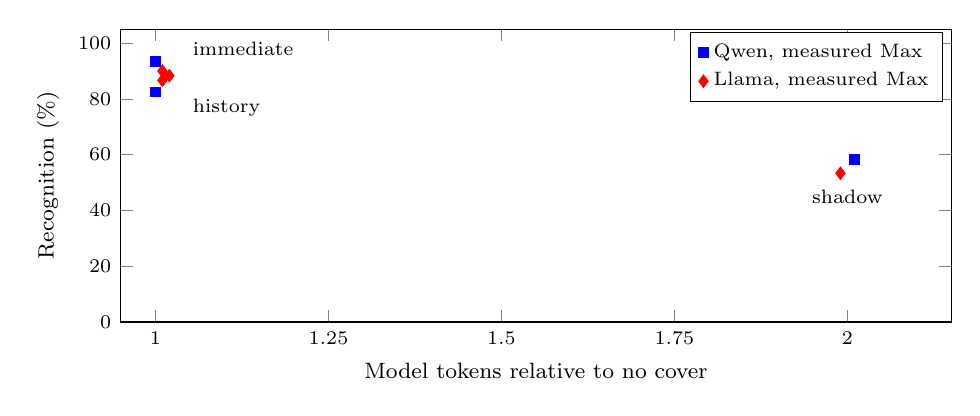
\begin{tikzpicture}
\begin{axis}[width=\columnwidth,height=5.3cm,xmin=0.95,xmax=2.15,ymin=0,ymax=105,
 xlabel={Model tokens relative to no cover},ylabel={Recognition (\%)},
 xtick={1,1.25,1.5,1.75,2},ytick={0,20,40,60,80,100},
 legend style={font=\scriptsize,at={(0.99,0.99)},anchor=north east,cells={anchor=west}},
 tick label style={font=\scriptsize},label style={font=\footnotesize}]
\addplot[only marks,blue,mark=square*,mark size=1.7pt] coordinates {(1,93.33) (1,82.5) (1,82.5) (2.01,58.33)};
\addlegendentry{Qwen, measured Max}
\addplot[only marks,red,mark=diamond*,mark size=2.2pt] coordinates {(1.01,90) (1.01,86.67) (1.02,88.33) (1.99,53.33)};
\addlegendentry{Llama, measured Max}
\node[font=\scriptsize,anchor=west] at (axis cs:1.04,98) {immediate};
\node[font=\scriptsize,anchor=west] at (axis cs:1.04,77) {history};
\node[font=\scriptsize,anchor=north] at (axis cs:2,51) {shadow};
\end{axis}
\end{tikzpicture}
\caption{Measured recognition and model work for the four cover policies. Points are strongest tested call-window attacks; overlapping controller points retain their values. Shadow changes call count and composition as well as model work. Ideal candidate-label values are shown separately in Table~\ref{tab:shadow-floor}.}\label{fig:frontier}
\end{figure}

